%%%% CAPÍTULO 3 - MATERIAL E MÉTODOS (PODE SER OUTRO TÍTULO DE ACORDO COM O TRABALHO REALIZADO)
%%
%% Deve apresentar o modelo utilizado, a modelagem
%% empregada, as simplificações necessárias, a
%% metodologia e a descrição do método de cálculo 
%% utilizado no desenvolvimento da pesquisa para que
%% a mesma possa ser reconstituída. Deve ainda 
%% apresentar resultados de amostras e comentários.
%% Deve apresentar a descrição da montagem 
%% experimental, metodologia para a obtenção de 
%% resultados, análise de erros, amostra de resultados
%% obtidos e comentários. Atenção: Esta parte pode ser
%% subdividida em mais capítulos de acordo com a 
%% especificidade do assunto.

%% Título e rótulo de capítulo (rótulos não devem conter caracteres especiais, acentuados ou cedilha)
\chapter{Material e Métodos}\label{cap:materialemetodos}

% Deve apresentar o modelo utilizado, a modelagem empregada, as simplificações necessárias, a metodologia e a descrição do método de cálculo utilizado no desenvolvimento da pesquisa para que a mesma possa ser reconstituída. Deve ainda apresentar resultados de amostras e comentários. Deve apresentar a descrição da montagem experimental, metodologia para a obtenção de resultados, análise de erros, amostra de resultados obtidos e comentários. Atenção: Esta parte pode ser subdividida em mais capítulos de acordo com a especificidade do assunto.



Para análise de desempenho da operação do transporte, é necessário incluir informação de tempo no modelo de rede utilizado. Em \cite{hol:12}, uma variedade de termos é apresentada para designar redes cuja estrutura é dependente do tempo: \emph{temporal graphs}, \emph{evolving graphs}, \emph{time-varying graphs}, \emph{time-aggregated graphs}, \emph{time-stamped graphs}, \emph{dynamic networks}, \emph{dynamic graphs}, \emph{dynamical graphs}, entre outros. O objetivo aqui não é discutir estes termos em profundidade, mas apenas destacar a ampla gama de opções para modelagem de redes dinâmicas. Particularmente, o modelo \emph{Time Varying Graph} (TVG) é adotado neste trabalho, tendo sido usado em \cite{sant:09}, além de \cite{tang:10} e \cite{lat:10} como uma sequência discreta e ordenada de grafos (a forma mais intuitiva de representação de um grafo variante no tempo). Um extensão dos conceitos clássicos de grafos para TVGs é apresentada em \cite{lat:12}. Em \cite{wach:19}, é apresentado um modelo TVG do transporte de ônibus de Greater Moncton no Canadá e sua implementação no banco de dados de grafos Neo4j\footnote{http://neo4j.org}. Conforme apontado em \cite{vick:10}, há um interesse crescente em bancos de dados noSQL (\emph{not only} SQL), como o Neo4j, para armazenamento e recuperação de dados com informação dinâmica.


 
 
%%%% reescrever e utilizar referências bibliográficas aqui >
% \ric{Aqui já tem muito detalhe para uma introdução}

% O Instituto de Pesquisa e Planejamento Urbano de Curitiba (IPPUC) descreve que o sistema de transporte coletivo da cidade de Curitiba como sendo composto por linhas urbanas e metropolitanas. Caracterizadas de acordo com sua função e categoria, as linhas de ônibus são diferenciadas por cores, conforme a descrição a seguir.
% \begin{itemize}
%     \item Expressas: constituem o sistema do transporte de massa na cidade. Transitam em vias próprias segregadas (os eixos estruturantes), possuem a cor vermelha e promovem a ligação dos terminais de integração à área central. Os ônibus são biarticulados (270 passageiros) ou articulados (180 passageiros) e suas paradas são constituídas por estações tubo; 
%     \item Alimentadoras: promovem a ligação dos terminais de integração aos bairros locais. Possuem a cor laranja e utilizam veículos com capacidades variadas, dependendo de sua demanda; 
%     \item Interbairros: interligam terminais e bairros de regiões diversas da cidade sem passar pela região central. De cor verde, utilizam veículos de capacidades variadas (110 a 160 passageiros);
%     \item Diretas: constituem linhas auxiliares às expressas e interbairros e promovem ligações pontuais mais distantes, com paradas médias a cada 3 km. Sua cor é prata e receberam o apelido de “ligeirinho”; 
%     \item Troncais: promovem a ligação dos terminais de bairro ao centro. De cor amarela, seus veículos possuem capacidade de 96 a 160 passageiros;
%   \item Intercidades: correspondem à ligação de municípios metropolitanos aos terminais urbanos. De cor laranja, seus veículos comportam 94 passageiros;
%  \item Convencionais: compreendem a ligação das áreas da cidade não atendidas pelos terminais de integração. Seus veículos são de cor amarela e possuem capacidade variável de 40 a 160 passageiros;
%   \item Circular Centro: promove a ligação de pontos do centro cidade. Utiliza-se de micro-ônibus na cor branca; 
%   \item Inter-hospitais: atendem um público que necessita deslocar-se entre hospitais, clínicas e laboratórios próximos à área central da cidade. Com veículos na cor branca, seu layout é específico, com capacidade para 22 passageiros; 
%  \item Madrugueiros: atendem um público que desenvolve suas atividades noturnas, em períodos fora dos horários de operação do sistema; 
%   \item Sites: correspondem às linhas do Sistema Integrado de Ensino Especial e atendem às escolas destinadas a portadores de deficiência (física ou mental). Seus veículos promovem o transporte porta a porta, ou seja, buscam seus usuários em suas casas e os levam às instituições de ensino a que se destinam, passando por um terminal de integração. Todos os veículos são adaptados às condições de seus usuários;
%   \item Aeroporto (executivo): promove a ligação do Aeroporto Internacional Afonso Pena à área central da capital com micro-ônibus na cor prata. 
% \end{itemize}


% Os terminais de integração correspondem à ligação das linhas que compõem a chamada RIT (Rede Integrada de Transporte) no município de Curitiba e também na região metropolitana. Esses terminais têm o objetivo de atender a população moradora das regiões vizinhas, que chegam até um dos 21 terminais da cidade por meio de linhas alimentadoras. No interior dos terminais é possível escolher qualquer percurso pagando uma tarifa única. Isso faz com que a população diminua gastos com o transporte. Os ônibus da Linha Expresso têm a função de complementar o trajeto até o centro da cidade por canaletas exclusivas. Curitiba conta ainda com linhas interbairros e linhas diretas que têm a finalidade de conectar outros pontos de Curitiba.

%  Assim como as linhas do transporte público são divididas em categorias, os terminais também recebem uma classificação. Os terminais  são divididos em: terminais de ponta, terminais intermediários, terminais de bairros, terminais de área central e terminais metropolitanos. Tal divisão, como o nome sugere, indica a posição dos mesmos no sistema de transporte, conforme ilustra a Figura ~\ref{fig:terminais}.
%  \begin{figure}[!h]
%  \caption{Localização e classificação dos terminais de ônibus de Curitiba}
%      \centering
%      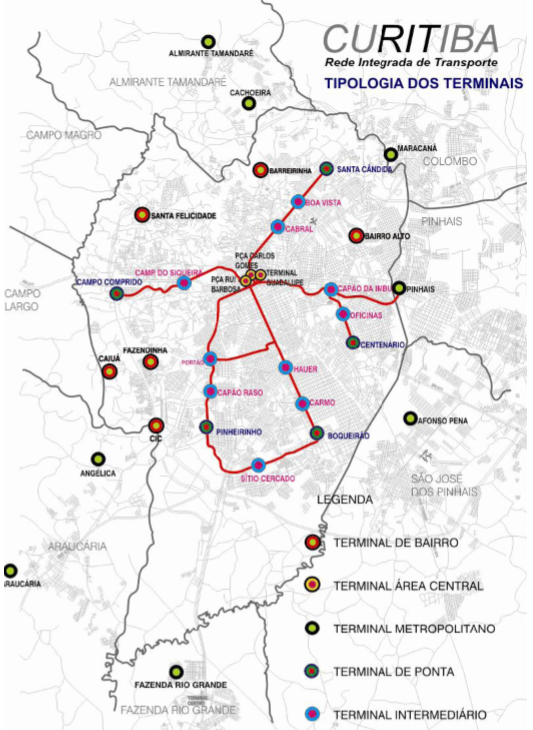
\includegraphics[scale=.95]{./Capitulo1/img/terminais.png}
%          \label{fig:terminais}
%      \fonte{Plano de Mobilidade Urbana de Curitiba, IPUCC 2019}
%  \end{figure}
 
%  %% << rever
 
% Na organização do artigo, a Seção~\ref{sec:fund} contém conceitos básicos e trabalhos relacionados. A Seção~\ref{sec:met} apresenta o modelo proposto. A Seção~\ref{sec:metr} define as métricas de redes complexas. A Seção~\ref{sec:impl} descreve a plataforma computacional desenvolvida. A Seção~\ref{sec:result} apresenta os resultados obtidos das métricas computadas para o transporte de Curitiba a partir do banco de dados de grafos. Conclusões e trabalhos futuros estão na Seção~\ref{sec:conclu}.


\section{Modelo Proposto} \label{sec:met}

O modelo proposto para o transporte público de Curitiba é mostrado na Figura~\ref{fig:model}. Este modelo tem por base o modelo de~\cite{wach:19}, com a inclusão do vértice \emph{Vehicle} para reduzir parte das informações sobre os veículos (ônibus) utilizados nas viagens que eram incluídas como atributos em vértices e arestas. A Figura~\ref{fig:model} mostra um grafo com vértices temporais (\emph{Schedule}, \emph{Trip} e \emph{Line}) e espaço-temporais (\emph{BusStop} e \emph{Stop}). Os vértices temporais carregam informações que variam com o tempo, enquanto os vértices espaço-temporais possuem informações de tempo associadas a dados de posicionamento georreferenciado. Vértices adicionais definem agrupamentos temporais do modelo que permitem recuperar informações para diferentes escalas de tempo (\emph{Year}, \emph{Month}, \emph{Day} e \emph{Hour}). Em resumo, o modelo da Figura~\ref{fig:model} representa dependências temporais e espaço-temporais entre os vértices do grafo que descreve a operação de um sistema de transporte.

\begin{figure}
\centering
\includegraphics[width=.8\textwidth]{fig/fig10.png}
\caption{Modelo TVG da movimentação dos ônibus do transporte.}
\label{fig:model}
\end{figure}



Os atributos dos vértices do grafo da Figura~\ref{fig:model} são mostrados nas Tabelas~\ref{tab:vertice_trip}, \ref{tab:vertice_vehicle}, \ref{tab:vertice_schedule}, \ref{tab:vertice_busstop}, \ref{tab:vertice_line} e \ref{tab:vertice_stop} do Apêndice. 
Cada linha de ônibus (vértices \emph{Line} - Tabela~\ref{tab:vertice_line}) dá origem a viagens (vértices \emph{Trip} - Tabela~\ref{tab:vertice_trip}). As viagens são programadas (vértices \emph{Schedule} - Tabela~\ref{tab:vertice_schedule}) para serem executadas por veículos (vértices \emph{Vehicle} - Tabela~\ref{tab:vertice_vehicle}), que geram sequências de movimentação e paradas (vértices \emph{Stop} - Tabela~\ref{tab:vertice_stop}). Estas paradas incluem paradas nos pontos de ônibus (vértices \emph{Bus Stop} - Tabela~\ref{tab:vertice_busstop}) para embarque e desembarque de passageiros. Além disso, as viagens possuem pontos de ônibus inicial, intermédiario(s) e final (vértices \emph{Bus Stop} - Tabela~\ref{tab:vertice_busstop}). Além disso, linhas de ônibus podem ser agrupadas e recuperados por dia (aresta \texttt{EXISTS\_LINE}), assim como paradas podem ser agrupadas e recuperadas por hora (aresta \texttt{EXISTS\_STOP}). Os atributos das arestas da Figura~\ref{fig:model} são mostrados na Tabela~\ref{tab:arestas} do Apêndice. As arestas estabelecem relacionamentos entre os vértices do grafo, além de carregarem atributos espaciais, temporais ou espaço-temporais para orientar consultas futuras.
Conforme será discutido na Seção~\ref{sec:impl}, a construção do grafo correspondente ao modelo da Figura~\ref{fig:model} no Neo4j é realizada a partir dos dados brutos da operação do transporte.

%Cabe ressaltar que o elemento do modelo que determina sua evolução dinâmica é os vértices do tipo \emph{Stop}, já que eles mapeiam as movimentações dos veículos ao longo do percurso definido pelas linhas e itinerários.




%\subsection{Vértices}

% Os vértices em roxo (\emph{year}, \emph{month}, \emph{day} e \emph{hour}) representam elementos essencialmente temporais representados. Tais elementos constituem a árvore temporal do grafo.

% Já os vértices em azul representam elementos temporais relacionados ao modelo de transporte, sendo constituído pelos seguintes vértices e seus respectivos atributos:

% Vértices em vermelho identificam vértices sem características temporais, sem características temporais ou espaço-temporais. Vértices em laranja identificam elementos espaço-temporais na rede, isto é, que possuem atributos de geolocalização assim como relações temporais.

% \textbf{Stop}: Identifica os pontos em que os veículos estiveram com velocidade inferior a 15Km/h. Pode ocorrer devido a paradas do veículo ou congestionamentos.
% \kei{imagino que seja um requisito a ser atendido pela linha (média de velocidade > 15km/h)}. Se a linha não a atende, deve ser registrada a causa (parada por problemas mecânicos e congestionamento mão usual). No cômputo da velocidade média deve considerar as paradas em pontos.

% \mar{Não entendi que conotação vc quer dar para a frase ``Pode ocorrer... congestionamentos'': no ponto de parada, idealmente a velocidade é zero, pois o ônibus pára para pegar ou deixar passageiros. Entretanto, na sua vizinhança, pode ocorrer congestionamento por conta de formação de comboios. Tb não se pode dizer que TODOs os pontos de parada geram congestionamentos. E tb não significa que o ônibus SEMPRE passará por ele a velocidade abaixo de 15km/h (ele pode passar direto pelo ponto se não tiver ninguém para pegar ou ninguém para deixar no ponto. Acho que é uma questão de formular mehor a frase.}

% \mar{Coloque uma referência para esse formato WKT.}

%\subsection{Arestas}

% As arestas conectam dois vértices de um grafo. Elas e seus atributos são descritos na Tabela~


% \begin{itemize}

% \item\textbf{EXISTS\_LINE}: Conecta a árvore temporal a existência da linha operante. Uma linha pode deixar de operar ao longo do tempo.

% \item\textbf{HAS\_TRIP}: Uma linha pode ter diversos sentidos: logo, esta aresta realiza a conexão da linha com os sentidos da linha.
% \item\textbf{HAS\_SCHEDULED\_AT}: Cada sentido da linha possui varios horários programados: logo esta aresta identifica a ligação entre os sentidos da linha e seus horários.
% \item\textbf{HAS\_VEHICLE\_SCHEDULED}: Esta aresta identifica os veículos que irão operar nos horários programados. Um veículo pode operar em mais de uma linha em horários diferentes.
% \item\textbf{HAS\_STOPPED}: Conecta um veículo a seu evento de parada.
% \item\textbf{STARTS\_ON\_POINT}: Conecta um sentido de linha a seu ponto de ônibus inicial determinando o início de seu roteiro.
% \item\textbf{HAS\_BUST\_STOP}: Identifica os pontos de ônibus que compõe um sentido da linha.
% \item\textbf{ENDS\_ON\_POINT}: Conecta um sentido de linha a seu ponto de ônibus final determinando o término de seu roteiro.

% \item\textbf{NEXT\_STOP}: Conecta dois pontos de ônibus em uma sequência.
% \begin{itemize}
%   \item\textbf{line\_code}: Código da linha.
%   \item\textbf{distance}: Distância em metros entre dois pontos de ônibus.
%   \item\textbf{service\_category}: Categoria da linha. 
%   \item\textbf{line\_name}: Nome da linha.
%   \item\textbf{card\_only}: Identifica se a linha aceita somente cartão como forma de pagamento.
%   \item\textbf{line\_way}: Identifica o sentido da linha.
%   \item\textbf{color\_name}: Cor da linha.
% \end{itemize}  

% \item\textbf{MOVED\_TO}: Liga a sequência de paradas de um determinado veículo.
% \begin{itemize}
%   \item\textbf{delta\_time}: Tempo em segundos entre duas paradas.
%   \item\textbf{delta\_distance}: Distância em metros entre duas paradas.
%   \item\textbf{delta\_velocity}: Velocidade média em metros por segundo entre duas paradas.
% \end{itemize}  

% \item\textbf{EVENT\_STOP}: Identifica um evento de parada de um veículo em uma área menor que 20 metros de um ponto de ônibus. Pode identificar que o veículo parou no ponto de ônibus.
% \begin{itemize}
%  \item\textbf{line\_way}: Sentido da linha que o ônibus seguia. 
% \end{itemize}  

% \end{itemize}


\section{Métricas de Redes Complexas} \label{sec:metr}

Uma vez que o grafo do sistema de transporte é modelado e armazenado no Neo4j, métricas de redes complexas podem ser computadas para avaliar o comportamento do sistema. Esta seção descreve as métricas utilizadas neste trabalho: i) centralidade de grau; ii) \emph{page rank}; iii) caminho mínimo e diâmetro; iv) centralidade de intermediação. Estas métricas foram escolhidas por permitirem uma avaliação da importância dos vértices na rede (pontos de ônibus), tanto do ponto de vista estático da topologia da rede quanto dinâmico da movimentação dos ônibus, e sua relação com os outros pontos da rede.

Proposto por \cite{free:79}, a {\bf centralidade de grau} é proporcional ao número de arestas (de entrada, ou de saída em grafos direcionados) que se conectam a um determinado vértice. Quanto maior a centralidade de grau de um vértice, maior é o número de conexões com outros vértices. No caso da rede de transporte, a centralidade de grau de um vértice \emph{Bus Stop} é proporcional ao número de paradas de ônibus no respectivo ponto para o caso dinâmico. Isso significa que pontos com elevada centralidade de grau podem corresponder a locais de potencial congestionamento ou de formação de comboios decorrente de uma estratégia de atendimento de demanda elevada. Para o caso estático, a centralidade de grau de um vértice \emph{Bus Stop} é proporcional ao número de linhas de ônibus que passam pelo vértice, já que apenas arestas para outros vértices \emph{Bus Stop} são consideradas.

O {\bf \emph{page rank}} foi concebido com o intuito de ranquear páginas (\emph{web sites}) relevantes da \emph{World Wide Web}. A ideia é que o fluxo de navegação dos usuários defina a relevância das páginas ao reforçar suas interconexões (\emph{hyperlinks}). O algoritmo PageRank \cite{brin:98} traduz a ideia intuitiva de que usuários em geral tendem a acessar páginas e navegar pela WWW usando \emph{hiperlinks} até uma certa profundidade. Assim, páginas bem posicionadas no fluxo de navegação são relevantes, pois tendem a ser muito visitadas pelos usuários. No contexto das redes de transporte, um ponto de ônibus com elevado \emph{page rank} pode indicar conexões com outros pontos importantes. Por exemplo, ligações diretas entre terminais de ônibus no caso estático.

O {\bf caminho mínimo} entre dois vértices é o caminho com o menor número de arestas, no caso de arestas não ponderadas. Caso as arestas tenham peso, deve-se considerar a soma dos pesos das arestas do caminho de um vértice a outro. A determinação de caminhos mínimos (considerando todos os pares de vértices de uma rede) é informação significativa para o planejamento urbano e a operação de um sistema de transporte, pois pode induzir no fluxo de pessoas na cidade. Algoritmos de caminho mínimo identificam rotas de conexão entre dois pontos da cidade de forma a minimizar o tempo de percurso necessário no transporte público \cite{Mart:2009, Larson:81}. Uma vez conhecidos os caminhos mínimos de todos os vértices para todos os outros da rede, define-se o {\bf diâmetro da rede} como o caminho mínimo mais longo da rede.

Introduzido por \cite{free:77} como uma medida para quantificar o controle de um ser humano sobre a comunicação entre outros seres humanos em uma rede social, a {\bf centralidade de intermediação} (\emph{betweenness centrality}) quantifica o número de caminhos que passam por um determinado vértice. Em outras palavras, a remoção de vértices com elevada centralidade de intermediação podem degradar ou mesmo interromper o fluxo de informação em uma rede. No contexto de sistemas de transporte, estes vértices são potenciais pontos de estrangulamento do sistema. Essa dependência pode ser temporal (ocorre em um intervalo de tempo específico) ou espacial (depende da posição espacial do ponto de ônibus), de acordo com o contexto da análise.




% \subsection{Conectividade}

% Conectividade é um propriedade que indica existe pelo menos um caminho entre todos os pares de vértices de uma rede. Caso não haja, existem sub-grafos isolados dentro da rede.

% No contexto das redes TVGs aplicadas ao sistema de transporte público, a evolução temporal desse sistema pode ou não gerar intervalos de tempo nos quais parte da rede perde conectividade com o restante da rede. Essa mudança na conectividade da rede pode ser um comportamento estrutural (ou seja, é um fenômeno recorrente da rede) ou uma anomalia (um fenômeno aleatório, como um acidente que bloqueie a passagem de veículos por uma via pública).


% \subsection{Centralidade de Grau}

% Proposto por \cite{free:79}, o grau de um vértice é o número de arestas (de entrada ou de saída) do vértice. Dependendo do contexto de análise, gargalos em redes podem estar relacionados a vértices com grau elevado.

% No caso do sistema de transporte, o grau é geralmente igual ao dobro do número de linhas que passam por um determinado ponto de parada de ônibus. Isso significa que pontos de parada com grau elevado podem corresponder a locais de potencial congestionamento ou de formação de comboios decorrente de uma estratégia de atendimento de elevada demanda.


%\subsection{Caminho mais curto}

% Define-se caminho entre dois vértices quaisquer como a sequência de vértices, ligados dois a dois por arestas, que deve ser percorrida para conectá-los. As arestas podem ser ponderadas ou não, definindo características das ligações entre dois vértice e afetando a definição do caminho. A partir dos caminhos existentes entre dois nós quaisquer, define-se como caminho mais curto aquele cujo ``esforço'' exigido para percorrê-lo é o menor dentre os caminhos existentes.

% Naturalmente, a determinação de caminhos e caminhos mínimos (considerando todos os pares de vértices existentes em uma rede) é informação significativa para planejamento dos usuários e dos operadores de um sistema de transporte como o de Curitiba, pois pode induzir no fluxo de pessoas pela cidade. Ao utilizar algoritmos de cálculo do caminho mais curto, pode-se identificar rotas de conexão entre dois pontos dentro da cidade de modo a minimizar o tempo a ser percorrido utilizando transporte público \cite{Mart:2009, Larson:81}.


%\subsection{Diâmetro e densidade de rede}

% Como consequëncia do cálculo de caminhos e caminhos mínimos, diâmetro (geodésico) de uma rede é o caminho mínimo mais longo dessa rede. Isso significa que há dois vértices cujo caminho mínimo é o mais longo a ser percorrido. Naturalmente, o contexto de análise pode implicar nesse diâmetro ser calculado a partir de atributos dos vértices e/ou arestas, como tempo exigido para percorrer dada par de vértice conectado, ou a distância entre esses pares de vértices conectados.

% Ja a densidade da rede mede a similaridade entre a rede e um grafo completo (grafo em que todos há um aresta para todos os seus pares de vértices) e pode ser definida como:

%  \begin{equation}
%      D = \mid E \mid / \mid N \mid ( \mid N \mid -1),
%  \end{equation} 
% na qual:

%  \begin{itemize}
%  \item $N$: é o número total de vértices.
%  \item $E$: é o número total de arestas.
% \end{itemize}  

% Neste artigo, a densidade da rede de trânsito é calculada em diferentes pontos e intervalos de tempo para identificar períodos intensa demanda do sistema de transporte (que geram picos de operação).


%\subsection{Centralidade de Intermediação}

% Introduzido por \cite{free:71} como uma medida para quantificar o controle de um ser humano sobre a comunicação entre outros seres humanos em uma rede social, a centralidade de intermediação quantifica quão importante um vértice (ou uma aresta) é na definição dos caminhos possíveis entre vários (ou todos) os pares de vértices de uma rede. Isso permite calcular qual a capacidade da rede se ``recuperar'' em caso de remoção de um ou mais vértices. Também é importante, pois auxilia na identificação de vértices que atuam como ``intermediários de serviços'' na rede.

% Para um vértice, a centralidade de intermediação é definida pela proporção dos caminhos que empregam um determinado vértice em relação a todos os caminhos existentes, ou seja:

%  \begin{equation}
%      B(u) = \sum_{s \neq u \neq t }^{} p(u) / p,
%  \end{equation} 
% na qual:

%  \begin{itemize}
%  \item $u$: é um vértice.
%  \item $p$: é o número total de caminhos entre os vértices $s$ e $t$.
%  \item $p(u)$: é o número de caminhos entre os vértices $s$ e $t$ que passam pelo vértice $u$.
% \end{itemize}  

% No contexto de sistemas de transporte, vértices com significativo $B$ são potenciais pontos de estrangulamento do sistema, dada a dependência que os caminhos possíveis desse sistema têm desse vértice. Essa dependência pode ser temporal (ocorre em um intervalo de tempo específico) ou espacial (depende da posição espacial do ponto de ônibus), de acordo com o contexto de análise.


% \subsection{Centralidade de PageRank}

% Com o intuito de ranquear as páginas (\emph{web sites}) mais significativos da \emph{World Wide Web}, o algoritmo Pagerank \cite{brin:98} foi concebido a partir das conexões existentes entre elas. A ideia intuitiva é que usuários em geral tendem a acessar páginas e navegar pela WWW usando os hiperlinks até uma certa profundidade. Assim, páginas que recebem muitas conexões devem ser muito significativas, pois devem ser muito visitadas pelos usuários.

% Usando o conceito presente em cadeias de Markov e/ou difusão em redes complexas, pode-se determinar os vértices mais significativos do ponto de vista de fluxos existentes em uma rede, quando o regime estacionário é atingido. Pode-se traduzir esse regime estacionário como a tendência de um usuário aleatório sempre chegar em uma determinada página, ou os dados em redes de comunicação sempre trafegarem por um determinado roteador.

% Neste artigo, a centralidade de PageRank é utilizada para quantificar a importância que as linhas e paradas de ônibus da rede de transporte público têm em diferentes intervalos de tempo (nos horários de alta demanda, ao longo do dia, ao longo do mês, por exemplo).



\section{Plataforma Computacional} \label{sec:impl}

A plataforma computacional desenvolvida gera um banco de dados de grafo no Neo4j a partir do \emph{dataset} diponibilizado pela operação do transporte coletivo de Curitiba.

% \ric{Na seção 2 tem o modelo formal; na seção 3 tem o modelo proposto implementado no Neo4j; nesta seção você mostra o dataset de entrada; precisa então detalhar como se dá a transformação do dadaset no modelo de dados do Neo4j; tem a Figura 2, mas não é auto-explicativa; precisa detalhar o que acontece; pelo menos para um exemplo.}

% Ao implementar modelo proposto, foram utilizadas diversas ferramentas e frameworks, esta seção se dispõe a descrever brevemente cada uma delas, assim como a arquitetura criada para ingestão dos dados em um banco de dados orientado a grafos.

% \mar{A frase acima precisa ser revista.}


\subsection{Dataset}

O portal de dados abertos de Curitiba fornece diariamente um \emph{dataset} em formato JSON (JavaScript Object Notation) com informações sobre o transporte coletivo da cidade. Conforme mencionado anteriormente, o transporte opera em média com uma frota de 1.410 ônibus que atende cerca de 1.389.731 passageiros por dia com 251 linhas de ônibus, 329 estações e 21 terminais.

A empresa URBS (gestora da Rede Integrada de Transporte Coletivo de Curitiba) define um conjunto de tabelas que contêm informações referentes às linhas de ônibus existentes, seus pontos de parada (que podem atender múltiplas linhas), os itinerários das linhas, os veículos que percorrem essas linhas, o percurso georeferenciado das linhas e o relacionamento entre essas informações. A descrição destas tabelas pode ser encontrada no dicionário de dados disponível no repositório de dados abertos. 
%\peix{Tais informações também estão disponíveis em forma de web service e pode ser acessado mediante a solicitação de login e senha. O dicionário de dados contendo a descrição das informações disponibilizadas pode ser obtido em \cite{dadosabertos}}

% Parte destes dados, que alimentam o fluxo de transformações descrito na Seção~\ref{subsec:work}, são detalhados nas Tabelas~\ref{tab:linhas}, \ref{tab:pontos_linha}, \ref{tab:tabela_veiculo} e \ref{tab:veiculos} do Apêndice.

%\ric{É preciso destacar pelo menos uma ou outra tabela mais importante.}

%\ric{Seria importante caracterizar também a dimensão desta base. Por exemplo, para 1 mês de captura de dados, estamos falando de qual volume de dados? Mostrar em uma tabela: número de linhas, viagens, ônibus, etc?}


% \ric{A Tabela~\ref{tab:data} mostra estatísticas do \emph{dataset} utilizado, com informações sobre o transporte coletivo de Curitiba coletados durante um mês de operação.}

% \begin{table}[h]
%     \caption{Estatísticas do \emph{dataset} do transporte de Curitiba para 1 mês de operação \mar{(qual mês/ano?)}.}
%     \label{tab:data}
%     \centering
%     \begin{tabular}{ccccc} 
%         \hline
%         No. de registros? &No. de linhas &No. de pontos &No. de ônibus &No. de viagens\\
%         \hline
%         xxx &xxx &xxx &xxx &xxx \\
%         \hline  
%     \end{tabular}
% \end{table}

%\ric{É IMPORTANTE? É importante salientar que essas tabelas apresentam redundâncias de dados, pois não foram normalizadas segundo preceitos de banco de dados. Isso significa que foi necessário pré-processá-lo para identificar e remover inconsistências.}


\subsection{Transformação do \emph{dataset} para a base de dados de grafo do Neo4j}
\label{subsec:work}

A Figura~\ref{fig:workflow} mostra o fluxo de transformação dos dados para a construção do modelo de grafo no Neo4j a partir do \emph{dataset} disponibilizado. Diversos fluxos foram implementados na linguagem Python usando as ferramentas Apache Airflow\footnote{https://airflow.apache.org/} e Apache Spark\footnote{https://spark.apache.org/}. 
%\mar{(checar se usou Python tb para Spark)}

\begin{figure}
\centering
\includegraphics[width=.9\textwidth]{fig/fig4.png}
\caption{Fluxos de transformação da fonte de dados para o banco de grafo.}
\label{fig:workflow}
\end{figure}


A primeira etapa consiste no carregamento dos dados brutos (em formato JSON) para uma área temporária de armazenamento (ou \emph{data lake}). Os arquivos JSON são transformados em arquivos parquet\footnote{https://parquet.apache.org/} \cite{Boufea:17} utilizando o Apache Spark. Arquivos parquet são formatos de armazenamento em colunas, otimizados para compressão e rápida recuperação de dados. 
%Nesta etapa é realizada somente a transformação de formato de arquivo e armazenamento de dados em uma área denominada data lake.
Na sequência, o conteúdo do \emph{data lake} é processado - também usando o Apache Spark - para gerar arquivos no formato CSV com os vértices e arestas do modelo de grafo apresentado na Seção~\ref{sec:met}. 

Embora vários fluxos de transformação de dados tenham sido implementados, detalha-se a seguir as transformações dos dados que criam o vértice \emph{Stop} e a aresta \texttt{EVENT\_STOP} do grafo. Estas estruturas modelam a dinâmica de movimentação dos ônibus e justificam o uso de um grafo variante no tempo.
%\mar{(Keiko e Ricardo: mexi nessa linha. Veja se melhorou.}

% O vértice \emph{Stop} é criado a partir da tabela \emph{VEICULOS} (Tabela~\ref{tab:veiculos} do Apêndice), que contém a geolocalização dos ônibus nos respectivos instantes de tempo. Com essa informação, calcula-se a distância percorrida, o tempo decorrido entre posicionamentos consecutivos e a velocidade média em km/h. Se a velocidade for menor do que 15 km/h, assume-se que houve uma parada do ônibus neste intervalo de tempo e um vértice \emph{Stop} é gerado no grafo com os respectivos atributos.

O vértice \emph{Stop} é criado a partir dos dados de geolocalização dos ônibus nos respectivos instantes de tempo (ver descrição da tabela \emph{VEICULOS} no dicionário de dados do repositório). Com essa informação, calcula-se a distância percorrida, o tempo decorrido entre posicionamentos consecutivos e a velocidade média em km/h. Se a velocidade for menor do que 15 km/h, assume-se que houve uma parada do ônibus neste intervalo de tempo e um vértice \emph{Stop} é gerado no grafo com os respectivos atributos.

% A aresta \texttt{EVENT\_STOP} é criada a partir dos vértices \emph{Stop} previamente obtidos das linhas dos ônibus, dos pontos de ônibus e da tabela horária dos ônibus nas linhas (Tabelas~\ref{tab:linhas}, \ref{tab:pontos_linha} e \ref{tab:tabela_veiculo} do Apêndice, respectivamente). Se uma parada (vértice \emph{Stop}) ocorrer a menos de 20 m de um ponto de ônibus (vértice \emph{Bus Stop}), considera-se que tal parada ocorreu em um ponto de ônibus e, portanto, cria-se uma aresta \texttt{EVENT\_STOP} para conectar os vértices \emph{Stop} e \emph{Bus Stop} no grafo.
% Uma vez construído o banco de dados de grafo para o transporte, consultas e análises de redes complexas podem ser realizadas a partir do Neo4j (\emph{Data Analysis} na Figura~\ref{fig:workflow}).

A aresta \texttt{EVENT\_STOP} é criada a partir dos vértices \emph{Stop} previamente obtidos das linhas dos ônibus, dos pontos de ônibus e da tabela horária dos ônibus nas linhas (ver descrição das tabelas \emph{LINHAS}, \emph{PONTOS\_LINHA} e \emph{TABELA\_VEICULO}, respectivamente, no dicionário de dados do repositório). Se uma parada (vértice \emph{Stop}) ocorrer a menos de 20 m de um ponto de ônibus (vértice \emph{Bus Stop}), considera-se que tal parada ocorreu em um ponto de ônibus e, portanto, cria-se uma aresta \texttt{EVENT\_STOP} para conectar os vértices \emph{Stop} e \emph{Bus Stop} no grafo.
Uma vez construído o banco de dados de grafo para o transporte, consultas e análises de redes complexas podem ser realizadas a partir do Neo4j (\emph{Data Analysis} na Figura~\ref{fig:workflow}).
 
